\documentclass[journal,10pt]{IEEEtran}

\usepackage{amsmath}
\usepackage{graphicx}
\usepackage{microtype}
\usepackage[hidelinks]{hyperref}
\hypersetup{
  pdftitle={Supplementary Material for Exact Robust Local Graph-Smoother Design Under Hidden-Topology Completions},
  pdfauthor={Che Lin}
}

% Generated by experiments.smoother.paper_data; do not edit by hand.
\newcommand{\CoreProblemCount}{54}
\newcommand{\CoreSamplingDesignCount}{270}
\newcommand{\PrincipalExactRadius}{0.808951}
\newcommand{\PrincipalUnboundedRadius}{1.000000}
\newcommand{\PrincipalFiniteGainPct}{19.1}
\newcommand{\PrincipalPSDTrueRadius}{0.891149}
\newcommand{\PrincipalPSDOverheadPct}{10.2}
\newcommand{\PrincipalSampleUnderMedianPct}{18.0}
\newcommand{\PrincipalSampleRegretMedianPct}{13.3}
\newcommand{\OneHopMedianGainPct}{18.7}
\newcommand{\FullPortMedianGainPct}{38.8}
\newcommand{\OneHopPSDMedianOverheadPct}{8.2}
\newcommand{\SamplingCurveRunCount}{420}
\newcommand{\SamplingCurveFailureCount}{420}
\newcommand{\SamplingWilsonLowPct}{88.6}
\newcommand{\PathWitnessCount}{3}
\newcommand{\PathMaxFinalRiskGap}{2.09\times 10^{-6}}
\newcommand{\PathMaxFinalBlockGap}{2.68\times 10^{-6}}
\newcommand{\PrincipalRounds}{1}
\newcommand{\PrincipalScalarHops}{6}
\newcommand{\PrincipalOnlineFlops}{16}
\newcommand{\PrincipalStorageBytes}{140}
\newcommand{\CrosscheckCount}{14}
\newcommand{\CrosscheckMaxRelativeRadiusDelta}{2.40\times 10^{-8}}
\newcommand{\CrosscheckMaxDeploymentRadiusDelta}{1.68\times 10^{-8}}
\newcommand{\CrosscheckMaxEpigraphGap}{6.45\times 10^{-10}}
\newcommand{\CrosscheckMaxLocalResidual}{3.05\times 10^{-11}}
\newcommand{\CorePrimaryOptimalCount}{40}
\newcommand{\CorePrimaryInaccurateCount}{14}
\newcommand{\CoreExactMedianTotalSeconds}{0.168}
\newcommand{\CoreExactMaxTotalSeconds}{4.13}
\newcommand{\CoreExactMaxQ}{5}
\newcommand{\CoreExactMaxH}{4}
\newcommand{\CoreMaxEpigraphGap}{4.63\times 10^{-8}}
\newcommand{\CoreMaxDeploymentRadiusChange}{6.31\times 10^{-9}}
\newcommand{\CoreMinDeployedCertificateEigenvalue}{-8.87\times 10^{-16}}


\title{Supplementary Material for ``Exact Robust Local\\
Graph-Smoother Design Under Hidden-Topology Completions''}
\author{Che Lin%
\thanks{Che Lin is an independent researcher (e-mail:
linmo891104@gmail.com).}}

\begin{document}
\maketitle

\section{Fixed-Known-Graph Local Algorithms}

This track deliberately studies a different task from robust completion
design: the full weighted graph is revealed and each method approximates that
one graph's smoother.  We average over random-cyclic, grid, geometric, and
small-world weighted graphs with 36 vertices and 16 graph-signal draws per
point.  Ordinary induced-neighborhood truncation, Neumann iteration, and
Chebyshev iteration all obey the stated causal radius, but truncation also
collects a local model and performs a local solve.  At four rounds, their mean
empirical MSEs are $8.63\times10^{-5}$, $6.69\times10^{-2}$, and
$5.95\times10^{-3}$, respectively; corresponding mean byte-hop counts are
426,972 for truncation and 79,360 for each polynomial method.  These are
graph-signal approximation errors, not WLS or Kalman measurement-noise MSEs.

\begin{figure*}[t]
  \centering
  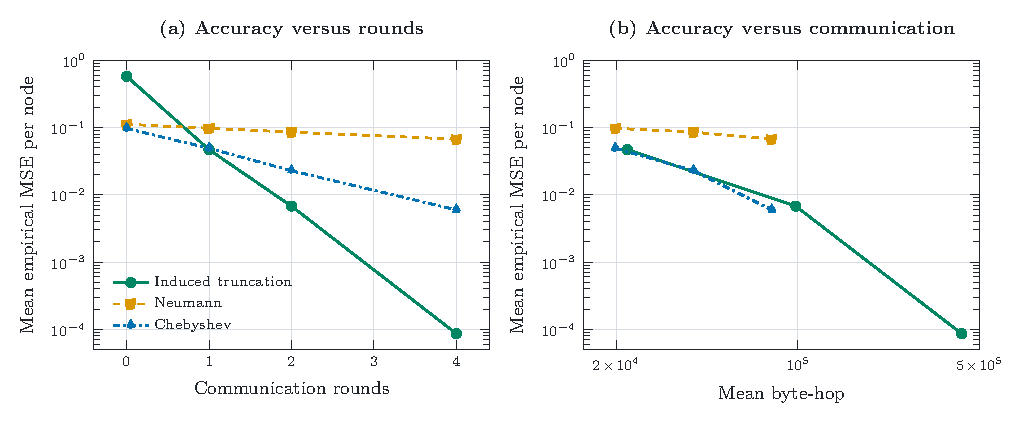
\includegraphics[width=\textwidth]{figures/local_method_tradeoff.pdf}
  \caption{Fixed-known-graph accuracy and communication tradeoff.  Induced
  truncation attains the lowest error in this small test but collects more
  model traffic; Chebyshev improves faster than Neumann at the same iterative
  byte-hop count.}
  \label{fig:local-tradeoff-supp}
\end{figure*}

\section{External Scale Stress Test}

Six PGLib-OPF v23.07 networks provide weighted topologies and three
SuiteSparse matrices provide symmetric sparsity graphs.  In every case the
benchmark constructs the unit-grounded matrix $I+L$; it does not reproduce or
claim the source dataset's original estimator.  The largest case has 129,164
vertices, and every sparse global-reference solve meets its configured
residual tolerance.  Figure~\ref{fig:external-stress-supp} records 16-round
Chebyshev relative signal error and reference-solve time.  Neither quantity is
converted into a theorem-matched hidden-completion certificate.

\begin{figure*}[t]
  \centering
  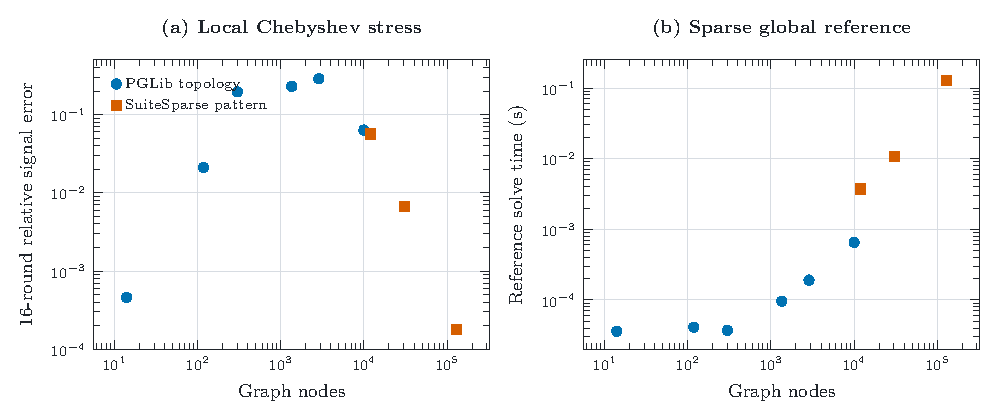
\includegraphics[width=\textwidth]{figures/external_stress.pdf}
  \caption{External graph-smoother stress tests.  PGLib cases contribute
  topology and positive branch weights; SuiteSparse cases contribute sparsity
  graphs.  Panel (a) reports 16-round Chebyshev relative signal error and panel
  (b) the sparse global-reference solve time.}
  \label{fig:external-stress-supp}
\end{figure*}

\section{Sampling Protocol and Metrics}

For each sampled rule $Q_N$, let $R_N(Q_N)$ denote the maximum full-input
operator-norm error over its $N$ training completions, and let $R_h(Q_N)$
denote the maximum over the complete finite-$h$ scenario set.  With $R_h^*$
the robust-design optimum, the reported quantities are
\begin{equation}
 u_N=\frac{R_h(Q_N)-R_N(Q_N)}{R_h(Q_N)},\qquad
 g_N=\frac{R_h(Q_N)}{R_h^*}-1.
\end{equation}
We declare underreporting when
$R_h(Q_N)-R_N(Q_N)>\max\{2\times10^{-5},10^{-3}R_h(Q_N)\}$.
The positive-contraction overhead uses the same ratio $g_N$ with $Q_N$
replaced by its baseline rule.

Each completion family cycles deterministically through random-cyclic, grid,
and geometric topologies, while hidden count cycles through $0,\ldots,h$.
Every nonzero edge weight is sampled log-uniformly on $[10^{-2},10^2]$; the
random-cyclic and geometric generators request mean degree four.  The breadth
grid uses five independently derived seeds and $N=32$ for each of 54 cells.
The budget study uses 30 independent base seeds for each of two problems and
nests sample prefixes for $N\in\{4,8,16,32,64,128,256\}$.  Its Wilson bounds
describe the 30 outcomes within a fixed problem and budget.  The empirical
CDFs pool grid evaluations without IID or population-inference claims: the
positive-contraction rule is reused across the three hidden budgets, and five
sampling seeds share each problem definition.

The positive-contraction baseline minimizes the same local-rule objective over
the outer uncertainty set $0\preceq X\preceq I$.  Its implementation uses the
lossless single-full-block Petersen LMI, including the scalar nonnegative
multiplier, and then reevaluates the returned $Q$ over every exact finite-$h$
scenario.  Thus its plotted value is finite-budget true risk, not the outer
set's optimization epigraph.

\section{Conic-Solver Postsolve Audit}

The fixed 54-problem core grid is solved with CVXPY 1.7.5 and the Clarabel
backend.  \CorePrimaryOptimalCount{} solves return \texttt{optimal} and
\CorePrimaryInaccurateCount{} return
\texttt{optimal\_inaccurate}.  We therefore do not use the conic epigraph
variable as the reported certificate: each returned matrix is thresholded at
relative magnitude $2\times10^{-5}$, then reevaluated directly over every
exact finite scenario.  Across the grid, the largest difference between the
solver epigraph and the recomputed squared risk is
$\CoreMaxEpigraphGap$, the largest radius change caused by deployment
thresholding is $\CoreMaxDeploymentRadiusChange$, and the smallest deployed
certificate eigenvalue is $\CoreMinDeployedCertificateEigenvalue$.  The
archived record contains each status,
active scenario, raw and deployed matrix, and all postsolve diagnostics.

This primal postsolve establishes the achieved radius and numerical
feasibility of each returned rule; by itself it does not turn an
\texttt{optimal\_inaccurate} status into a numerical optimality proof.  We
therefore rerun all \CrosscheckCount{} flagged cells independently with SCS
3.3.1 at \texttt{eps=1e-8}.  All return \texttt{optimal}.  After exhaustive
scenario reevaluation, the maximum relative radius disagreement with Clarabel
is $\CrosscheckMaxRelativeRadiusDelta$ (or
$\CrosscheckMaxDeploymentRadiusDelta$ after deployment thresholding); the
largest SCS epigraph--recomputed squared-risk gap is
$\CrosscheckMaxEpigraphGap$, and the largest local-rule residual is
$\CrosscheckMaxLocalResidual$.  This is numerical cross-solver corroboration,
not a rigorous dual lower bound.  Because $Q$ can vary along flat optimizer
directions, we compare objective radii and make no uniqueness claim for the
returned matrix.  Independently of
this audit, all nine one-hop state problems, the representative $q=4,h=1$
rule, and both exact references in the sampling-budget study already have
primary status \texttt{optimal}; every zero-hop constant-preserving problem
fixes $Q=I$.

\section{Hardware-Specific Accelerator Timing}

This experiment is separated from the main theorem-matched results because it
measures one implementation on one platform; it is neither a complexity claim
nor evidence for the completion theorem.  Three independent process runs
compare 40 rounds of a fixed local Richardson smoother on two-dimensional
grids.  OpenMP and OpenBLAS are restricted to one CPU thread, and the
accelerator is an NVIDIA RTX 5080.  Median resident-kernel speedups (CPU time
divided by GPU time) are $0.273$, $1.468$, $3.235$, and $69.38$ at 10,000,
50,176, 102,400, and 1,000,000 states, respectively.  Including vector
host--device transfers gives $0.259$, $1.400$, $2.922$, and $50.35$.  The
observed crossover therefore lies between 10,000 and 50,176 states on this
system.  The archived experiment record contains the three process-level
repetitions, package and platform versions, normalized configuration, and
source hash used to generate the figure.

\begin{figure*}[t]
  \centering
  
\includegraphics[width=0.78\textwidth]{figures/cpu_gpu_crossover.pdf}
  \caption{CPU/GPU crossover for a 40-round unit-grounded grid smoother.
  Curves show medians over three process runs, and the blue band spans the
  observed resident-kernel range.}
  \label{fig:cpu-gpu}
\end{figure*}

\end{document}
